\documentclass[11pt]{report}

\usepackage{times}
\usepackage{latexsym}
\usepackage{booktabs}
\usepackage{amsmath}
\usepackage{multirow}
\usepackage{enumitem}
\usepackage{amsfonts}
\DeclareMathOperator*{\argmax}{arg\,max}

\newcommand*{\checktikz}[1][]{\tikz[x=1em, y=1em]\fill[#1] (0,.35) -- (.25,0) -- (1,.7) -- (.25,.15) -- cycle;}

\newcommand{\Correct}{\checktikz[draw=black]}
\newcommand{\ValidMiss}{\checktikz[draw=gray,fill=white]}
\newcommand{\Valid}{\checktikz[draw=gray,fill=white]}
\newcommand{\Missed}{\checktikz[draw=black]} %\textsf{X}~}
\newcommand{\Wrong}{} %\textsf{X}~}

\usepackage[utf8]{inputenc}
\usepackage[letterpaper,bindingoffset=0.2in,%
            left=1in,right=1in,top=1in,bottom=1in,%
            footskip=.25in]{geometry}
\usepackage{microtype}
\usepackage{mathtools}
\usepackage{latexsym, mathrsfs}
\usepackage{graphicx}
\usepackage{subcaption}
\usepackage[usenames,dvipsnames,svgnames,table]{xcolor}
\usepackage[framemethod=TikZ]{mdframed}
\usepackage[linesnumbered,ruled,procnumbered]{algorithm2e}
\usepackage{enumitem}
\usepackage{multirow}
\usepackage{xspace}
\usepackage{textcomp}
\usepackage{setspace}
\usepackage{tikz}
\usepackage{hhline}
\usepackage[numbers,sort]{natbib}
\usepackage[nottoc]{tocbibind}
\usepackage[normalem]{ulem}
\usepackage[titletoc]{appendix}

\usepackage{titlesec}
\titleformat{\chapter}
  {\normalfont\LARGE\bfseries}{\thechapter}{1em}{}
\titlespacing*{\chapter}{0pt}{3.5ex plus 1ex minus .2ex}{2.3ex plus .2ex}

% VQuel listing
\newcommand{\mysinglespacing}{%
  \setstretch{1}% no correction afterwards
}


\usepackage[pdfpagelabels=false]{hyperref}
\hypersetup{
   colorlinks,
   linkcolor={red!50!black},
   citecolor={blue!50!black},
   urlcolor={blue!80!black}
}

\SetAlFnt{\small}

\mdfdefinestyle{MyFrame}{%
    linecolor=black,
    outerlinewidth=1pt,
    roundcorner=10pt,
    innertopmargin=\baselineskip,
    innerbottommargin=\baselineskip,
    innerrightmargin=20pt,
    innerleftmargin=20pt,
    backgroundcolor=gray!50!white}
    
\newenvironment{denselist}{
    \begin{list}{\small{$\bullet$}}%
    {\setlength{\itemsep}{0ex} \setlength{\topsep}{0ex}
    \setlength{\parsep}{0pt} \setlength{\itemindent}{0pt}
    \setlength{\leftmargin}{1.5em}
    \setlength{\partopsep}{0pt}}}%
    {\end{list}}

\usepackage{cleveref}
\crefname{section}{\S\!\!\!\;}{\S\S}
\Crefname{section}{\S}{\S\S}

\RequirePackage{natbib}
% for citation commands in the .tex, authors can use:
% \citep, \citet, and \citeyearpar for compatibility with natbib, or
% \cite, \newcite, and \shortcite for compatibility with older ACL .sty files
\renewcommand\cite{\citep}	% to get "(Author Year)" with natbib    
\newcommand\shortcite{\citeyearpar}% to get "(Year)" with natbib    
\newcommand\newcite{\citet}	% to get "Author (Year)" with natbib   

\newcommand{\topic}[1]{\vspace{-3.5pt}\smallskip \smallskip \noindent{\bf #1:}}
\newcommand{\stitle}[1]{\vspace{0.5em}\noindent\textbf{#1}}
\renewcommand{\stitle}[1]{\vspace{1em}\noindent\textbf{#1}}

\newcommand{\speaker}[1]{{\bf\footnotesize\textsf{#1}}}
\renewcommand{\vec}[1]{\boldsymbol{#1}}

%COMPRESS
\newcommand{\squeezeup}{\vspace{-2.5mm}}

\newcommand{\U}{\mathbb{U}}

\title{
{\bf Teaching Machines to Ask Clarification Questions}\\
\vspace{18pt}
\it Preliminary Oral Exam (Thesis Proposal)}

\author{
{\bf Sudha Rao}  \\
Department of Computer Science \\
University of Maryland, College Park\\
{\texttt{raosudha@cs.umd.edu}}
}


\date{
\vspace{42pt}
Dissertation Proposal submitted to: \\
Department of Computer Science \\
University of Maryland, College Park, MD 20742 \\
\bigskip
\bigskip
\today
\bigskip
\bigskip
\begin{table}[htp]
\begin{center}
\begin{tabular}{lll}
&\multicolumn{2}{l}{Advisory Committee:} \\ \\
Dr. Hal Daum\`{e} III & Chair & U. of Maryland, College Park \\
Dr. David Jacobs & Dept's Rep & U. of Maryland, College Park \\
Dr. Philip Resnik & Member & U. of Maryland, College Park \\
Dr. Lucy Vanderwende & Member & Microsoft Research \\
\end{tabular}
\end{center}
\end{table}%
}


\begin{document}

\pagestyle{plain}
\pagenumbering{roman}

\maketitle
\pagebreak

\begin{abstract}
\normalsize

Inquiry is fundamental to communication, and machines cannot effectively collaborate with humans unless they can ask questions. Asking questions is also a natural way for machines to express uncertainty, a task of increasing importance in an automated society. In the field of natural language processing, despite decades of work on question answering, there is relatively little work in question asking. Moreover, most of the previous work has focused on generating reading comprehension style questions which are answerable from the provided text. The goal of my dissertation work, on the other hand, is to teach machines to ask clarification questions pointing out the missing information in a text. Primarily, I focus on two scenarios where I find such question asking to be useful: (1) clarification questions on posts found in community-driven Q\&A forums like StackExchange (2) clarification questions during goal-oriented dialogue sessions. 

In my first line of research, I study the problem of question generation using data from StackExchange, a plentiful online resource in which people routinely ask clarifying questions to posts so that they can better offer assistance to the original poster. In my preliminary work, I created a novel dataset using StackExchange and addressed the question selection problem, more specifically select the right clarification question from a set of prior questions. I developed a novel neural network model inspired by the notion of expected value of perfect information: a good question is the one whose expected answer is going to be the most useful. In my first proposed work, I plan to use the following two strategies to build more generalizable systems: (a) a template based question generation model and (b) an encoder-decoder based neural generative model.

In my second line of research, I study the problem of question generation using the Ubuntu Dialogue Corpus, a two-way conversational data extracted systematically from chat logs where people discuss issues with their Ubuntu Operating system. In my preliminary work, I addressed the task of predicting the next best response given a context of a conversation. I built a novel neural network model inspired by the best practices in dialogue modeling coupled with our novel vocabulary selection strategies. In my second proposed work, I plan to explore how can I generate a clarification question as the next response, given different levels of context of a conversation. 

In both the research agendas described so far, I took a purely corpus-driven approach to generating clarification questions i.e. learning to ask a question by looking at previously asked questions in a similar context. However, inferring a knowledge gap requires a certain level of domain knowledge that is currently lacking in our proposed models. Therefore, in my third proposed work, I plan to explore how can we use external knowledge sources to understand what is missing in a given context and then ask a clarification question. 

\end{abstract}

\pagebreak

\tableofcontents
\pagebreak

\cleardoublepage
\pagenumbering{arabic}


\chapter{Introduction}

\section{Motivation}

An overarching goal of the natural language processing community is to develop techniques that would enable machines to process naturally occurring text as efficiently as humans do. However, as humans, we do not always understand each other. In pragmatics, Grice's theory of conversational implicatures \cite{grice1975logic} says that there is a difference between what someone says and what someone `implicates' by uttering a sentence. What someone says is determined by the conventional meaning of the sentence uttered and contextual processes of disambiguation; what she implicates is associated with the existence of some rational principles and maxims governing conversation. The Gricean maxims of conversation says that speakers and listeners adhere to a Cooperative Principle where a speaker communicates information that is as informative as required and not more. The speaker assumes a certain common ground or mutual information or shared knowledge with the listener \cite{clark1991grounding,clark1982hearers,clark1981definite}. In case of gaps or mismatches in knowledge, the listener resorts to asking questions. Correction of such knowledge deficits has been identified as one of the key purposes of asking questions \cite{graesser2008question}. \\

\noindent
With the advancements of artificial intelligence technologies, automated agents like Apple's Siri, Amazon's Alexa, Google Assistant, etc are becoming increasingly common in our day-to-day lives. We might use these agents to say set up an alarm, check for the weather OR schedule a meeting. However, many-a-times these agents fail to understand what we tell them presumably due to a mismatch in the common knowledge we assume with them. If we wish to make such human-bot interactions as efficient as human-human interactions are, it is important that we teach machines to ask clarification questions when faced with uncertainty or knowledge gaps.\\

\noindent
In the field of natural language processing, however, despite decades of work on question answering, there has been little work in question asking. Moreover most of the previous work on generating questions has been on generating reading comprehension style questions: given a text, write a question that one might find on a standardized test assessing the knowledge of a student about a particular topic in the text. Comprehension questions, by definition, are answerable from the provided text. Clarification questions are not. The goal of this thesis work is to explore how can a machine automatically generate clarification questions when faced with uncertainty or knowledge gaps. 

\section{Research questions}

About a decade ago, if you faced a technical problem the only way to solve it would be to go to an expert. Due to the recent surge in the use of internet, a lot of such problem solving these days happen online on question answering (Q\&A) forums where users post their problems and other users reply to them providing assistance. However, \newcite{asaduzzaman2013answering} observed that on StackExchange, which is one such community-driven problem solving platforms, many a times the posts go unanswered for a long time because they are not clear enough i.e. they are missing some information. Consequently, other users ask clarification questions to those posts so that they can better offer assistance to the original poster. Our first research question is the following: \textit{Can we build a model that can learn to automatically generate a clarification question to a post by looking at clarification questions posted in the forum before?}\\

\noindent
Human-bot interaction has become increasingly popular in recent times. Apple's siri, Amazon's alexa, Google Home, IBM's watson are all examples of successful advancements in the artificial intelligence technology. These technologies are great when it comes to simple natural language based interactions like ``What is the weather like in New York City?'' OR ``Play me latest top 10 songs'', etc. However when one tries to use these interfaces for more complicated purposes like ``I can't start my laptop. Help me\!'', OR ``Find me a recipe for lasagne'', within a few interactions one would soon give up. One key reasons for such failures is the lack of common understanding between the human user and the bot. The human user has a certain understanding of the problem/request he has and many a times he fails to convey the same understanding to the bot. In such a scenario, the bot can be much more useful if it could try to establish this common understanding by asking relevant questions. Our second research question is the following: \textit{Can we build an interactive model that can learn to ask clarification questions when faced with uncertainty or a knowledge gap?}\\

\noindent
% clarification question with the help of knowledge base i.e. find out what is missing and then ask a question

\section{Proposed solutions}

In order to learn how to ask clarification questions, we build a model inspired by the decision theoretic framework of expected value of perfect information (EVPI). EVPI is a measurement of the value of gathering information. A good question is the one whose likely answer is going to be the most useful. In our setting, we use EVPI to calculate which question is most likely to elicit an answer that would make the post more informative. On StackExchange, users routinely ask clarification questions to post. The author of the post subsequently edits the post answering the question. We mine many (post, question, answer) triples using StackExchange's edit histories. We extract the initial post as p, question posted in the comments section as q, and edit to the original post as answer a to form our (p,q,a) triples. Using this data, we build our EVPI inspired neural network model which learns to ask a clarification question given a post.\\

\noindent
In our preliminary work, we focus on the question selection problem i.e. select the right clarification question from a set of prior questions. Given a post, we first generate a set of candidate questions by identifying posts similar to the given post and then looking at the questions asked to those posts. For identifying similar posts, we use Lucene \footnote{https://lucene.apache.org/}, a software extensively used in information retrieval for extracting documents relevant to a given query from a pool of documents. To enable our system to generalize better on new unseen cases, we propose two research directions: a template based question generation method where we first generate templates and then fill in the variables using the current context of the post; and a sequence-to-sequence based neural generative model where we generate the question one word at a time given a post. \\

\noindent
We study the problem of clarification question generation in a dialog setting using the Ubuntu Dialog corpus, a large corpus recently put together by \newcite{lowe2015ubuntu} by extracting two-way conversations from chat logs where people were discussing about the issues they were having with the Ubuntu Operating system. In our preliminary work, we consider the problem of next utterance classification i.e. given a context of a conversation and a set of possible next responses, choose the correct next response. Recently, \cite{serban2016multiresolution} proposed a multi-resolution recurrent neural network model where they generate the high-level coarse tokens like nouns, entities and activities using a separate layer in their model thus indirectly giving more importance to the topic words in a conversation. \\

\noindent
Our model, on the other hand, that captures a similar notion using what we call the `bursty vocabulary' i.e. we up-weight the words that occur frequently within the short context of a conversation, thus avoiding the need for manually crafting the list of coarse tokens. We build a novel neural network based model that combines several best practices in dialogue modeling such as utterance level hierarchy, attention, character trigram histograms and context based vocabulary selection strategy. This approach gives us significant improvements over current neural network baselines. In our next step, we propose to look at the responses in the conversations that are questions and build a model that learns to generate a question based response given different levels of context of a conversation. We will combine both the template based approach and the neural generative approach described before to generate the question based response. \\

\noindent
Finally, in our last proposed work, we plan to explore how can we make use of external knowledge sources to determine what information is missing in the given context and then ask a question probing for that missing information. Traditional dialogue systems \cite{lemon2006isu} can be viewed as methods for slot-filling where a question is generated during a dialogue specifically with the purpose of filling a set of slots defined in a structured knowledge base. On the contrary, in our work, we are interested in using unstructured knowledge sources like the Wikipedia to identify a missing information. We plan to use the domains of StackExchange such as academia, music, mythology, etc where participating in the Q\&A requires quite a lot of background knowledge. Our clarification question generation model for posts on these domains will then extract relevant information from Wikipedia before it generates a question. 

\section{Organization}

Chapter~\ref{background} presents a review of the current methods for question generation, a review of the neural network models used in natural language processing tasks and finally a review of the current methods for dialogue modeling. 
Chapter~\ref{stackexchange} describes our preliminary work on generating clarification questions for posts on StackExchange. Chapter~\ref{dialogue_next_response} describes our preliminary work on dialogue modeling where we develop a neural network model for generating next response given the context of a conversation. Chaper~\ref{proposed_work} describes our three proposed work extending our preliminary work on clarification question generation. Chaper~\ref{conclusion} concludes our proposal and describes a timeline for our remaining proposed works.

\newpage

\chapter{Background}\label{background}

\section{Question Generation}

Question generation received its first wide-spread attention during the Question Generation shared task \cite{rus2010first,rus2011question}. This work recognized question generation as an essential component of learning environments, help systems, information seeking systems, multi-modal conversations between virtual agents, etc. It defined the task as question generation from sentences and paragraphs. \cite{vanderwende2008importance} point out that the focus of evaluation in such tasks should not just be the grammaticality of the generated questions but also the \textit{importance} of the generated questions.  \cite{heilman2011automatic} describe approaches for generating factual reading comprehension questions: given text, write questions that one might find on a standardized test. \cite{olney2012question} tackle the same problem under the context of tutoring systems. They generate a concept map (graph with topic terms as nodes and relations between topic terms as edges) and then define rules to generate questions using these maps. \cite{labutov2015deep} generate high-level question templates by crowdsourcing and given a text segment, rank question templates that are relevant.

 \cite{liu2010automatic} generate template based questions to help author write better related work sections. Input to their system is a literature review and output is a set of questions. Their system captures all the citations referred in a paper, extract features out of it and then uses fixed templates to ask questions about the content. \cite{mostafazadeh2016generating} introduce a Visual Question Generation task where they consider question generation from images, a multi-modal variant of question generation. Their work differs from image captioning as the generated question in their case helps infer something from the image that is not explicitly shown in the image. \cite{penas2010filling} identify the notion of missing information similar to us but they attempt to fill the knowledge gaps in a text with the help of external knowledge bases; whereas we try to generate a question that would point at the missing information. \cite{artzi2011bootstrapping} use human-generated clarification questions to drive a semantic parser where the clarification questions are aimed towards simplifying a user query.

\section{Neural networks in natural language processing}

Neural networks are powerful machine learning models that have recently achieved excellent performances on speech recognition \cite{hinton2012deep} and visual object recognition tasks \cite{krizhevsky2012imagenet}. Feedforward Neural Networks \cite{bebis1994feed}, Recurrent Neural Networks \cite{medsker2001recurrent}, Gated Recurrent Neural Networks \cite{bahdanau2014neural}, etc are some of the variations of this idea. \cite{lecun2015deep} give us a brief review of the neural network models. In the field of natural language processing, a version of such neural networks called the Long Short Term Memory \cite{hochreiter1997long} that can capture long range dependencies has shown to be powerful for many language based tasks. The basis of these neural networks is a vector based representation for words \cite{mikolov2013distributed,pennington2014glove} that capture the distributional semantics learnt from a huge corpus of text. 

Neural network methods have proved to be useful for a number of natural language processing tasks in recent times. \cite{bengio2003neural} present a neural probabilistic language model. \cite{mikolov2010recurrent} introduce recurrent neural network based language model.\cite{bahdanau2015neural} show the power of an attention-based neural network model for the task of machine translation where they jointly learn to align and translate words of sentences between two languages. \cite{iyyer2014neural} introduce a neural network model for factoid question answering over paragraphs. \cite{hermann2015teaching} teach machines to read and comprehend using neural networks. 

\section{Dialogue modeling}

Understanding dialogues require us to detect the inherent discourse structure in them. Although this is a hard problem, there is some agreement that a useful first step is to identify what is called the Dialogue Acts or Speech Acts \cite{searle1969speech}. \cite{stolcke2000dialogue} have shown that the dialog acts can be used for the automatic tagging and recognition of conversational speech. The first work that spurred a wide-spread interest in dialogue modeling was the Dialog State Tracking Challenge \cite{williams2013dialog}. \cite{lemon2006isu} introduce dialog systems with the purpose of filling the slots of a knowledge base. One particular challenge with data-driven approaches to the problem of dialogue modeling was the dearth of publicly available datasets. 

Recently, \cite{lowe2015ubuntu} introduced a large Ubuntu Dataset Corpus by systematically extracting two-way conversations from chat forums where people were discussing issues they had with their Ubuntu Operating Systems. In our work, we use this data for our preliminary task of next utterance classification in a dialogue context. \cite{lowe2015ubuntu}  introduced a baseline model for this problem using a long short-term memory (LSTM) neural network model. \cite{xu2016incorporating} incorporate domain knowledge by enhancing their LSTM model with a recall gate. \cite{serban2016hierarchical} introduce a latent variable hierarchical recurrent encoder-decoder model by adding a context level RNN that processes sequences of sub-sequences operating on top of the token level RNN. \cite{serban2016multiresolution} take a similar hierarchical approach but instead of defining a latent coarse representation, they assume it to be observed and experiment with two such representations (sequence of nouns and sequence of activities and entities). \cite{yao2016attentional} have shown that attending to the context while generating the words of the response, similar to attention based model used for machine translation, gives an improvement over using just the last hidden state. Recently, \cite{bordes2016learning} introduced an end-to-end approach for goal oriented dialog systems. \cite{pappu2014knowledge} describe a knowledge acquisition strategy for similar goal-oriented dialog systems. 

\newpage

\chapter{Clarification Questions for Question-Answering Forums}\label{stackexchange}

\section{Introduction}\label{introduction}

A main goal of asking questions is to fill information gaps, typically through clarification questions, which naturally occur in conversations. 
A good question is one whose \emph{likely answer} is going to be most useful.
Consider the exchange in Figure~\ref{askubuntu_post}, in which an initial poster (who we'll call ``Terry'') asks for help configuring environment variables.
This question is underspecified and a responder (``Parker'') asks a clarifying question ``\textsf{\small (a) What version of Ubuntu do you have?}''
Parker could alternatively have asked one of:

\textsf{\small(b) Is the moon waxing or waning?}

\textsf{\small(c) Are you running Ubuntu 14.10 kernel 4.4.0-59-generic on an x86\_64 architecture?}

\noindent
Parker should not ask (b) because it's not useful; they should not ask (c) because it's too specific and an answer of ``No'' gives little help.
Parker's question (a) is optimal: it is both likely to be useful, and is plausibly answerable by Terry.
Our goal in this paper is is to automate Parker.
Specifically, after Terry writes their initial post, we aim to generate a clarification question so that Terry can immediately amend their post in hopes of getting faster and better replies.
\begin{figure}
\centering
\setlength\fboxsep{1pt}
\setlength\fboxrule{0.5pt}
\fbox{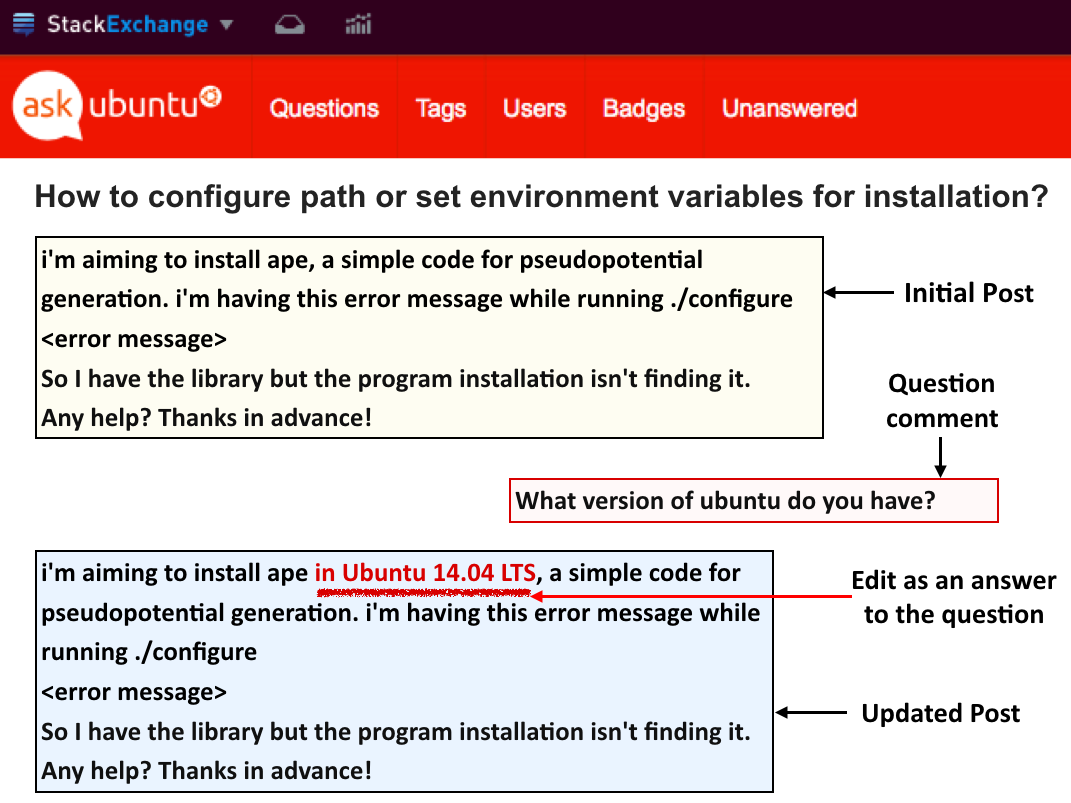
\includegraphics[width=0.47\textwidth]{askubuntu_post}}
\caption{A post on an online Q \& A forum ``askubuntu.com'' is updated to fill the missing information pointed out by the question comment}
\label{askubuntu_post}
\end{figure}
%
Our work has two main contributions: 
\begin{enumerate}[noitemsep,nolistsep]
%\item Identifying the problem of generating clarification questions as a problem worth of study, both in its own right and as part of the larger problem of building naturalistic conversational systems. 
\item A novel neural-network model for addressing this task that integrates the notion of expected value of perfect information (\S\ref{model}). % , a classic formalization from AI
\item A novel dataset, derived from StackExchange, that enables us to learn a model to ask clarifying questions by looking at the types of questions people ask (\S\ref{dataset_creation}).\footnote{We use data from StackExchange; per license cc-by-sa 3.0, the data is ``intended to be shared and remixed'' (with attribution). We will release all of the data we extract.}
\end{enumerate}

To develop our model we take inspiration from the decision theoretic framework of the Expected Value of Perfect Information (EVPI), a measure of the value of gathering additional information. In our setting, we use EVPI to calculate which question is most likely to elicit an answer that would make the post more informative.
Formally, for an input post $p$, we want to choose a question $q$ that maximizes $\mathbb{E}_{a \sim p,q}[\U(p+a)]$, where $a$ is a hypothetical answer and $U$ is a utility function measuring the \emph{completeness} of post $p$ if $a$ were to be added to it.
To achieve this, we construct two models:
(1) an answer model, which estimates $\mathbb{P}[a~|~p,q]$, the likelihood of receiving answer $a$ if one were to ask question $q$ on post $p$;
(2) a completeness model, $\U(p)$, which measures how complete a post is.
Given these two models, at prediction time we search over a shortlist of possible questions for that which maximizes the EVPI.

We are able to train these models jointly based on $(p,q,a)$ triples that we extract automatically from StackExchange.
Figure~\ref{askubuntu_post} depicts how we do this using StackExchange's edit history.  In the figure, the initial post fails to state what version of Ubuntu is being run. In response to Parker's question in the comments section, Terry, the author of the post, edits the post to answer Parker's clarification question. We extract the initial post as $p$, question posted in the comments section as $q$, and edit to the original post as answer $a$ to form our $(p,q,a)$ triples. 

Our results show significant improvements from using the EVPI formalism over both standard feedforward network architectures and bag-of-ngrams baselines, even when our system builds on strong information retrieval scaffolding. In comparison, without this scaffolding, the bag-of-ngrams model outperforms the feedforward network. We additionally analyze the difficulty of this task for non-expert humans, and give examples of system output. 

\section{Related Work} \label{related_work}

The problem of question generation has received sparse attention from the natural language processing community. Most prior work focuses on generating reading comprehension questions:  given text, write questions that one might find on a standardized test \cite{vanderwende2008importance,heilman2011automatic,rus2011question,olney2012question}.  Comprehension questions, by definition, are answerable from the provided text. Clarification questions are not.  

Outside reading comprehension questions, \newcite{labutov2015deep} generate high-level question templates by crowdsourcing and given a text segment, rank question templates that are relevant. However the crowdsourcing method of collecting data leads to significantly less data than we collect using our method. \newcite{liu2010automatic} use template question generation to help authors write better related work sections. \newcite{mostafazadeh2016generating} introduce a Visual Question Generation task where they consider question generation from images, a multi-modal variant of question generation. 
\newcite{penas2010filling} identify the notion of missing information similar to us but they attempt to fill the knowledge gaps in a text with the help of external knowledge bases, whereas we instead ask clarification questions. \newcite{artzi2011bootstrapping} use human-generated clarification questions to drive a semantic parser where the clarification questions are aimed towards simplifying a user query; whereas we generate clarification questions aimed at  identifying missing information in a text. 

\section{Model description}\label{model}

In order to choose what question to ask, we build a neural network model inspired by the theory of expected value of perfect information (EVPI). EVPI is a measurement of: if I were to acquire information X, how useful would that be to me? However, because we haven't acquired X yet, we have to take this quantity in expectation over all possible X, weighted by each X's likelihood. In the question generation setting, for any given question $q$ that we can ask, there is set $A$ of possible answers that could be given. For each possible answer $a \in A$, there is some probability of getting that answer, and some utility if that were the answer we got. The value of this question $q$ is the expected utility, over all possible answers. The theory of EVPI then states that we want to choose the question $q$ that maximizes:
\begin{equation}\label{evpi_equation}
\argmax_{q \in Q} \sum_{a \in A} \mathbb{P}[a | p,q] \U(p+a)
\end{equation} 

In Eq~\ref{evpi_equation}, $p$ is the post, $q$ is a potential question from a set of candidate questions $Q$ and $a$ is a potential answer from a set of candidate answers $A$. $\mathbb{P}[a | p,q]$ measures the probability of getting an answer $a$ given an initial post $p$ and a clarifying question $q$. $\U(p+a)$ is a utility function that measures how useful it would be if $p$ were augmented with answer $a$. In our case, the utility function we use is the completeness of the post: a post has high utility the more complete it is. This captures the right intuition in the example questions (from Section~\ref{introduction}) that Parker could have asked such that: \textsf{\small (a)} will have good utility for many likely answers;
\textsf{\small (b)} will have low utility regardless of the answer; and
\textsf{\small (c)} will have high utility only for a low probability answer.

The modeling question then is how to model: 
\begin{enumerate}[noitemsep,nolistsep]
\item the probability distribution $\mathbb{P}[a | p,q]$ and
\item the utility/completeness function $\U(p+a)$.
\end{enumerate}
In our work, both will be represented using neural networks over the appropriate inputs. Posts, questions and answers will all be represented as embeddings. We train the parameters of the two models jointly to minimize a joint loss defined such that an answer that has a higher potential of increasing the utility of a post gets a higher probability.

\begin{figure*}[t]
\centering
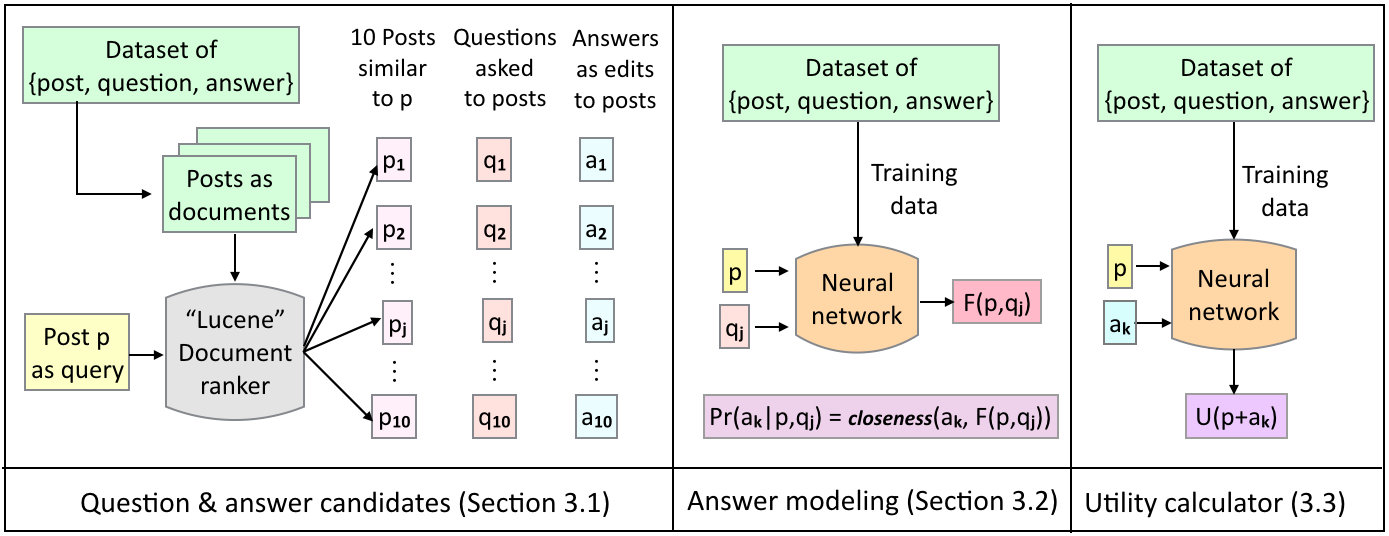
\includegraphics[width=0.85\textwidth]{model}
\caption{\small The behavior of our model during test time. Given a post $p$, Lucene retrieves 9 posts similar to post $p$ and consider the questions asked to those 9 posts, plus the original, as question candidates. The edits made to the posts in response to the questions as our answer candidates. For each question candidate $q_i$, we generate an answer representation $F(p,q_j)$ and calculate how close is the answer candidate $a_k$ to our answer representation $F(p,q_j)$. Our utility calculator calculates the utility of the post if it were updated with the answer $a_k$. Finally we return the question $q$ that maximizes the expected utility of the post $p$ (Equation~\ref{evpi_equation}).}
\label{model}
\end{figure*}

Figure~\ref{model} describes the behavior of our model during test time. 
Given a post $p$, our first step is to generate a set of candidate questions and a set of candidate answers (Section~\ref{question_candidate_generator}).
Given a post $p$ and a question candidate $q_i$, our second step is to calculate how likely is this question to be answered using one of our answer candidates $a_k$ (Section~\ref{answer_modeling}).
Given a post $p$ and an answer candidate $a_k$, the third step is to calculate the utility of the updated post i.e. $\U(p + a_k)$ (Section~\ref{utility_calculator})
Finally, using these pieces, we build a joint neural network that we can optimize end-to-end over our data (Section~\ref{neural_network}).

\subsection{Question \& answer candidate generator}\label{question_candidate_generator}

Given a post $p$, our first step is to generate a set of candidate questions and a set of candidate answers. One way that humans learn to ask questions is by looking at how others ask questions in a similar situation. Using this intuition we generate question candidates for a given post by identifying posts similar to the given post and then looking at the questions asked to those posts. For identifying similar posts, we use Lucene\footnote{\url{https://lucene.apache.org/}}, a software extensively used in information retrieval for extracting documents relevant to a given query from a pool of documents. Lucene also ranks the extracted documents according to their relevance to the query. We use Lucene to find the top 10 most similar posts to a given post from our dataset (Section~\ref{dataset_creation}) \footnote{The top most similar candidate to a post is the original post itself}. We consider the questions asked to these 10 posts as our set of question candidates and the edits made to the posts in response to the questions as our set of answer candidates. Section~\ref{dataset_creation} describes the process of extracting the (\textit{post, question, answer}) triples from the StackExchange datadump. 

\begin{figure*}[ht]
\centering
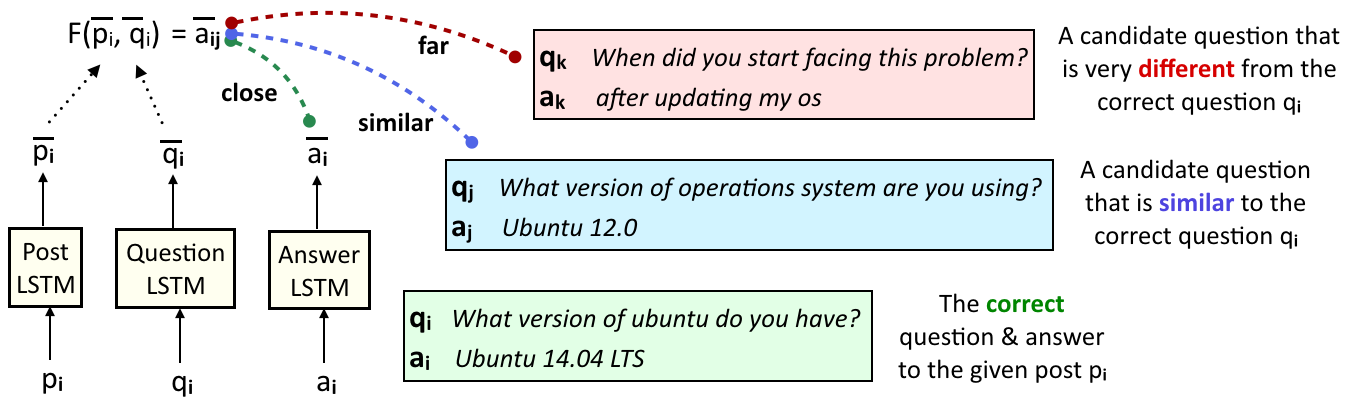
\includegraphics[width=0.9\textwidth]{answer_generator}
\caption{Training of our answer generator. Given a post $p_i$ and its question $q_i$, we generate an answer representation that is not only close to its correct answer $a_i$, but also close to one of its candidate answers $a_j$ if the candidate question $q_j$ is close to the true question $q_i$.}
\label{fig_answer_generator}
\end{figure*}

\subsection{Answer modeling}\label{answer_modeling}

Given a post $p$ and a question candidate $q_i$, our second step is to calculate how likely is this question to be answered using one of our answer candidates $a_k$. To calculate this probability, we first generate an answer representation using $p$ and $q_i$ and then measure how close is the answer candidate $a_k$ to our answer representation. To model our answer generator we use the following intuition: a question can be asked in several different ways. For e.g. in Figure~\ref{askubuntu_post}, the question ``\textsf{\small What version of Ubuntu do you have?}'' can be asked in other ways like ``\textsf{\small What version of operating system are you using?}'', ``\textsf{\small Version of OS?}", etc.  
Additionally, for a given post and a question, there can be several different answers to that question. For instance, ``\textsf{\small Ubuntu 14.04 LTS}", ``\textsf{\small Ubuntu 12.0}", ``\textsf{\small Ubuntu 9.0}", are all valid answers. We train our answer generator to generate an answer representation capturing these generalizations.

We use our dataset of \{\textit{post, question, answer}\} triples (Section~\ref{dataset_creation}). Given a $\{p_i, q_i, a_i\}$ triple, we use a long short-term memory architecture (LSTM) \cite{hochreiter1997long} to get to their respective neural hidden representations $\{\bar p_i, \bar q_i, \bar a_i\}$.  Given $(\bar p_i, \bar q_i)$, we define a feed-forward neural network $F$ that combines the post and question representations to get an answer representation $F(\bar p_i, \bar q_i)$. We train our answer generator to minimize the loss function below:
%
\begin{align}\label{eq_answer_generator}
  \textrm{loss}_{\textrm{ans}}(\bar p, \bar q, \bar a, Q) 
  &=  {|| F(\bar p, \bar q) - \bar a||}^2 & \\
  &\hspace{-25mm} +  \sum_{j \in Q} \Big ( {|| F(\bar p, \bar q) - \bar{a_j} ||}^2  (1 - \tanh{(|| \bar q - \bar{q_j} ||^2)}) \Big ) \Big \} &\nonumber
\end{align}
%
This loss function can be explained using the example in figure~\ref{fig_answer_generator}. Question $q_i$ is the question paired with the given post $p_i$. In equation~\ref{eq_answer_generator}, the first term forces the function $F(\bar p_i, \bar q_i)$ to generate an answer representation as close as possible to the correct answer $a_i$. Now, a question can be asked in several different ways. Let $Q_i$ be the set of candidate questions for post $p_i$, retrieved from the dataset using Lucene (Section~\ref{question_candidate_generator}). Suppose a question candidate $q_j$ is very similar to the correct question $q_i$ ( i.e. $|| \bar q_i - \bar{q_j} ||$ is near zero). Then the second term forces the answer representation $F(\bar p_i, \bar q_i)$ to be close to the answer $a_j$ corresponding to the question $q_j$ as well. Thus in the figure~\ref{fig_answer_generator}, the answer representation will be close to $a_j$ (since $q_j$ is similar to $q_i$), but far off from $a_k$ (since $q_k$ is dissimilar to $q_i$).

Given such an answer representation, we then define the probability distribution over candidate answers $a_k \in A$ as: 
\begin{align}
\mathbb{P}[a_k |p_i,q_j]  
&= \frac 1 Z \exp\left[- \lambda || a_k  -  F(p_i,q_j) ||^2\right]
\end{align}
where $\lambda$ is a tunable parameter that controls the variance of the distribution.

\subsection{Utility calculator}\label{utility_calculator}
Given a post $p$ and an answer candidate $a_k$, the third step is to calculate the utility of the updated post i.e. $\U(p + a_k)$. As expressed in equation~\ref{evpi_equation}, this utility function measures how useful it would be if a given post $p$ were augmented with an answer $a_k$. We train our utility calculator using our dataset of \{\textit{post, question, answer}\} triples (Section~\ref{dataset_creation}). We label all the $(p_i, a_i)$ pairs from our triples dataset with label $y=1$. To get negative samples, we make use of the answer candidates generated using Lucene as described in Section~\ref{question_candidate_generator}. For each $a_k \in A_i$, where $A_i$ is the set of answer candidates for post $p_i$, we label the pair $(p_i, a_k)$ with label $y=0$, except for when $a_k == a_i$. Thus, corresponding to each post $p_i$ in our triples dataset, we get one positive sample and nine negative samples. 

Given a post $p$ and an answer $a$, we use a post LSTM and an answer LSTM to get the neural representation $\bar{p}$ and $\bar{a}$. We define a feedforward neural network that combines the post neural representation $\bar{p}$ and the answer neural representation $\bar{a}$ to get the updated post representation $F(\bar{p}, \bar{a})$. The utility of the updated post is then defined as $\U(p+a) = \sigma ( F(\bar{p}, \bar{a}) )$. We want this utility to be close to 1 for all the positively labelled $(p,a)$ pairs and close to 0 for all the negatively labelled $(p, a)$ pairs. We therefore define our loss using the binary cross-entropy formulation below:
%
\begin{align}\label{eq_utility_calculator}
  \textrm{loss}_{\textrm{util}}(y, \bar p, \bar a) &= y \log(\sigma (F(\bar{p}, \bar{a})))
\end{align}

\subsection{Our joint neural network model}\label{neural_network}
Our fundamental representation is based on recurrent neural networks over word embeddings. We obtain the word embeddings using a GloVe \cite{pennington2014glove} model trained on the entire datadump of StackExchange. Given an initial post $p$, we generate a post neural representation $\bar{p}$ using a post LSTM i.e. long short-term memory architecture \cite{hochreiter1997long} as shown in the figure~\ref{lstm}. Similarly, given a question $q$ and an answer $a$, we generate a question neural representation $\bar{q}$ and a answer neural representation $\bar{a}$ using a question LSTM and an answer LSTM respectively. We define the function $F$ as a feedforward neural network on its input with two fully-connected hidden layers. So the function $F(\bar{p},\bar{q})$ in our answer model would be a feedforward neural network on the inputs $\bar{p}$ and $\bar{q}$ and the function $F(\bar{p}, \bar{a})$ in our utility calculator would be a feedforward neural network on the inputs $\bar{p}$ and $\bar{a}$. We train the parameters of the three LSTMs corresponding to $p$, $q$ and $a$, and the parameters of the two feedforward neural networks jointly to minimize the sum of the loss of our answer model (Eq~\ref{eq_answer_generator}) and our utility calculator (Eq~\ref{eq_utility_calculator}):
%
\begin{align}
                       \sum_i \textrm{loss}_{\textrm{ans}}(\bar p_i, \bar q_i, \bar a_i, Q_i)  
                        +  \textrm{loss}_{\textrm{util}}(y_i, \bar p_i, \bar a_i)
\end{align}
%
Given such an estimate $\mathbb{P}[a|p,q]$ of an answer and a utility $\U(p+a)$ of the updated post, predictions (i.e., selecting a question from a set of candidate questions) can be done by choosing that ``$q$'' that maximizes Eq~\ref{evpi_equation}. The remaining question, then, is how to get data that enables us to train our answer model and our utility calculator. Given data, the training becomes a multitask learning problem, where we learn simultaneously to predict utility and to estimate the probability of answers.

\begin{figure}
\centering
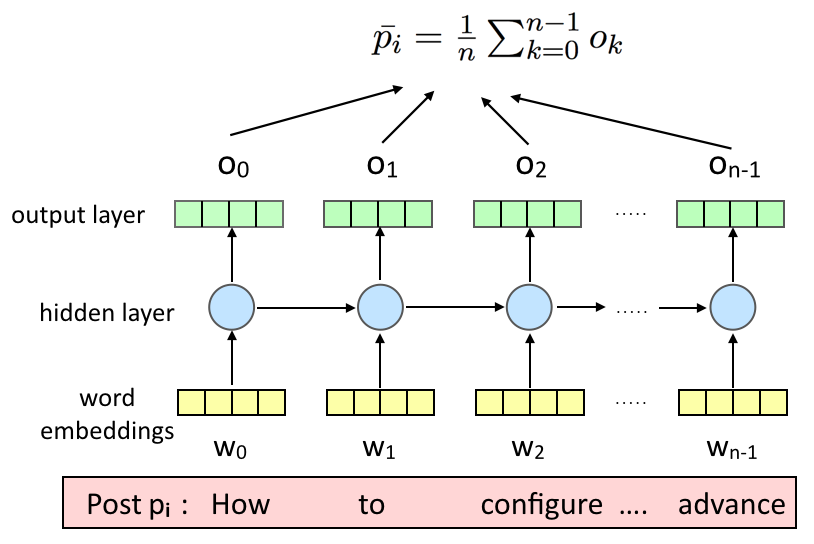
\includegraphics[scale=0.27]{lstm}
\caption{{\small Our LSTM architecture on a post $p_i$. The input layer consists of pre-trained word embeddings of the words in the post which is fed into a single hidden layer. The output $o_k$ of each of the hidden states is averaged together to get our neural representation $\bar p_i$}}
\label{lstm}
\end{figure}

\section{Dataset creation}\label{dataset_creation}
StackExchange is a network of online question answering websites about varied topics like academia, ubuntu operating system, latex, etc. The sites are modeled after StackOverflow, a popular platform used for asking and answering questions on a wide range of topics in computer programming. The data dump of StackExchange contains timestamped information about the posts, comments on the post and the history of the revisions made to the post. We use this data dump to create our dataset of \{\textit{post, question, answer}\} triples: where the \textit{post} is the initial unedited post, the \textit{question} is the comment containing a question and the \textit{answer} is the edit made to the post that matches the question comment. \\
\textbf{Extract posts:} We use the post histories to identify posts that have been updated by its author. We use the timestamp information to retrieve the initial unedited version of the post.\\
\textbf{Extract questions:} For each such initial version of the post, we use the timestamp information of its comments to identify the first comment made to the post. We look for a question mark `?' token to further identify if its a question comment. Finally, we truncate the comment till the question mark token to retrieve the question part of the comment.\\
\textbf{Extract answers:} In our final step, we identify the edit made to the post in response to the question comment. Authors make edits to their posts for several reasons; including stylistic updates and grammatical corrections. Therefore, we use only those edits that are longer than four words and finally use the timestamp information of the edit to match the edits to their respective question comments.

We extract a total of 38,041 (\textit{post, question, answer}) triples from StackExchange which are distributed across three domains: askubuntu (13,749), unix (6656), and superuser (17,636). We train our models using 80\% of the data, tune our hyper parameters using 10\% of the data and evaluate our models using the remaining 10\% of the data. Table~\ref{data_statistics} shows the sizes of the train, dev and test splits for the three domains. 

\begin{table}
\centering
\begin{tabular}{lccc}
\toprule
& Train & Dev & Test  \\
\midrule
askubuntu & 10,992 & 1374 & 1375\\
unix & ~~~5324 & ~~666 & ~~666 \\
superuser & 14,828 & 1404 & 1404 \\
\bottomrule
\end{tabular}
\caption{Table above shows the sizes of the train, dev and test split of our dataset for three domains.}
\label{data_statistics}
\end{table}

A natural question to our process of data creation would be how often is the extracted question a clarification question. We sample a set of 1400 questions from our dataset and design a crowdsourced task where given a question we ask a human to choose whether: a) It is a clarification question, b) It provides an answer or a suggestion; or c) Neither.  63\% of the questions are marked as clarification question, 33\% of them are marked as questions that provides an answer or a suggestion and 4\% of them are marked as neither. The inter-annotator agreement (PAA) is above 90\%. These numbers suggest that although a greater percentage of the extracted questions are clarification questions, our data is imperfect: it includes some non-clarification questions.

\section{Experimental Results}\label{experiments_results}
Our primary research questions that we evaluate experimentally are:
%
\begin{enumerate}[noitemsep,nolistsep]
\item Does a neural architecture with learned representations improve upon a simple bag-of-ngrams baseline?

\item Does the expected value of perfect information (EVPI) formalism provide leverage over a similarly expressive feed-forward network? %In particular, is EVPI a useful inductive bias for a model?

\item In the EVPI formulation, is it useful to compute an expectation over answers, rather than just picking a single question/answer pair?

\item How well does our model perform in comparison to non-expert humans?

\item How much harder is the task when the (distrator) candidate questions come from Lucene rather than selected randomly?\footnote{A common strategy with the Ubuntu dialogue corpus \cite{lowe2015ubuntu} is to train a dialogue system by choosing a best response given a context of a conversation and a set of candidate responses. However, these methods generate their candidates from their dataset using random sampling. This plausibly makes the task significantly easier than using Lucene to select candidates, which are much more likely to be confusable and have high lexical overlap.}
\end{enumerate}

\begin{table*}[t]
\small
\centering
\begin{tabular}{l|cccc|cccc}
\toprule
 & \multicolumn{4}{c|}{Lucene negative candidates} & \multicolumn{4}{c}{Random negative candidates} \\
Models & Acc & MRR & R@3 & R@5 & Acc & MRR & R@3 & R@5\\
\midrule
Random  & 10.0 & 29.3 & 30.0 & 50.0 &10.0 & 29.3 & 30.0 & 50.0 \\
Bag-of-ngrams & 11.6 & 31.3 & 32.5 & 54.6 & 54.9 & 70.5 & 83.1 & 92.0 \\
Feed-forward & 17.4 & 37.8 & 43.2 & 63.9 &  49.0 & 66.8 & 81.3 & 92.8 \\
EVPI max  & 21.1 & 41.2 & 48.0 & 66.9  & 48.8 & 65.5 & 77.2 & 89.9 \\
EVPI sum & \bf 23.3 & \bf 43.4 & \bf 51.0 & \bf 70.3 & \bf 61.1 & \bf 75.5 & \bf 87.9  & \bf 95.8  \\
\bottomrule
\end{tabular}
\caption{Results of our two setups `Lucene negative candidates' and `Random negative candidates' on askubuntu test split when the model is trained on a combination of askubuntu, unix and superuser train splits}
\label{results_topN}
\end{table*}


\subsection{Task setups}\label{task_setup}

\textbf{Lucene negative candidates:} In this setup, given a post $p$, we label the question $q$ paired with $p$ in our dataset of $(p, q, a)$ triples as positive. To get our negative candidates, we retrieve nine additional question candidates using Lucene (as described in Section~\ref{question_candidate_generator}).\\
\textbf{Random negative candidates:} In this setup, given a post $p$, we label the question $q$ paired with $p$ in our dataset of $(p, q, a)$ triples as positive as in the previous setting. To get our negative candidates, we randomly sample nine other questions from our dataset of $(p, q, a)$ triples.\footnote{In all cases we train 100-d word embeddings using GloVe \cite{pennington2014glove} on the 3 billion token datadump of StackExchange. We use a threshold frequency of 100 to create our vocabulary of ~250,000 tokens. For our feed-forward neural network, we use two fully-connected dense hidden layers each of size 100. We use ReLU \cite{nair2010rectified} non-linearity as our activation function between the hidden layers.}


\subsection{Baseline methods}\label{baselines}

We compare our model with the following baselines:\\
\textbf{Random baseline:} Given a post, we randomly permute its set of 10 candidate questions uniformly.\\
\textbf{Bag-of-ngrams baseline:} Given a post and a set of 10 question question and answer candidates, we construct a bag-of-ngrams representation for the post, the question and the answer. Our bag-of-ngrams baseline is then trained to minimize hinge loss on misclassification loss using cross-product features between each of (\textit{post, question}), (\textit{question, answer}) and (\textit{post, answer}). We tune the ngram length and the learning rate and choose the setting that performs best on development data.\\
\textbf{Neural network baseline using post, question and answer:} We concatenate the post LSTM representation, the question LSTM representation and the answer LSTM representation and feed it through a feed forward neural network of two fully-connected hidden layers to get our neural baseline. 

\subsection{Dataset}\label{dataset}
We evaluate our model and our baselines on the following three domains of StackExchange: askubuntu, unix and superuser.
 \begin{description}
 \item[askubuntu:]  A question and answer site for users of the Ubuntu Operating system where people post queries about issues they face while using Ubuntu. An example question on this site: ``\textsf{\small Why isn't Chromium up-to-date in all the Ubuntu LTS repos, like Firefox is?}''
 \item[unix:]  A question and answer site for users of Linux, FreeBSD and other unix-like operating systems. This site would contain questions like the ones in askubuntu and more. An example question on this site: ``\textsf{\small How to repeatedly alternate between two (or more) commands?}''
 \item[superuser:] A question and answer site for users of all kinds of operating systems and computer applications. An example question on this site: ``\textsf{\small What is the LAST version of Windows Operating system that can run DOS applications natively?}''
 \end{description}

Table~\ref{data_statistics} shows the data statistics for the four sites above.  Although StackExchange consists of many sites, we choose the ones above because: a) The data dump available for them were moderately big in size to train a model on; b) These domains contain clarifications questions that are generic enough to be useful for many different posts; and finally c) The three domains were close enough so that we could combine them to create our full dataset of ~37K triples.

\subsection{Results}

We first describe results on the union of all data, summarized in Table~\ref{results_topN}.
We report four metrics: accuracy (percent of time the top ranked question was correct),
mean reciprocal rank (the reciprocal of the ranked position in the top ten list that the correct question is), 
recall at 3 (percent of the the correct answer is in the top three) and
at 5.

The left half of this table shows results when the candidate sets is from Lucene---the ``hard'' setting.
Here, we see that for all the evaluation metrics:
EVPI using the sum (expectation over $a$) outperforms
EVPI using the max $a$;
which outperforms the neural feedforward model that does not incorporate the EVPI formalism;
which outperforms the bag-of-ngrams baseline;
which outperforms the random baseline.
The gains in all cases are relatively large: at least a few percentage points.
A final performance of 51\% recall at 3 is encouraging, though clearly there is a long way to go for a perfect system.

The right half of this table shows the same results when the candidate set is chosen randomly---the ``easy'' setting.
A major difference in the results here is that the bag-of-ngrams system now \emph{outperforms} both the feedforward neural model and the EVPI using max instead of expectation.
This likely happens because just picking up on word overlap---when Lucene has not already done this for us---works remarkably well.
Nonetheless, in all of the metrics, the true EVPI model outperforms all the baselines, achieving at least a 3\% gain over the bag-of-ngrams baseline.

In Table~\ref{results_topM}, we show results when we work not with the union of all the data, but with each data set individually.
%The top half is against Lucene candidate, the bottom half is against random candidates.
The main observation is that the trends are essentially the same as before: for Lucene negative candidates, bag-of-ngrams underperforms feedfoward, which underperforms EVPI.
This happens because more data helps, and these three domains are sufficiently similar that the additional data---even if it is slightly domain mismatched---is better than nothing.
%The second observation is that the results for EVPI are lower across the board, with the exception of superuser on random negative examples.% (which is sometimes better, sometimes worse).

\begin{table*}
\footnotesize
\centering
\begin{tabular}{l|cccc|cccc|cccc}
\toprule
&  \multicolumn{12}{c}{Lucene negative candidates}\\
 & \multicolumn{4}{c|}{askubuntu} & \multicolumn{4}{c|}{unix} & \multicolumn{4}{c}{superuser}\\
Models & Acc & MRR & R@3 & R@5 & Acc & MRR & R@3 & R@5 & Acc & MRR & R@3 & R@5\\
\midrule
Bag-of-ngrams  & ~~7.0 & 25.1 & 22.5 & 40.7&  4.5 & 22.9 & 19.6 & 38.7&  6.5 & 25.2 & 22.6 & 42.8\\
Feedforward & 13.3 & 33.4 & 36.1 & 57.3  & 13.4 & 32.7 & 34.0 & 56.6  & 14.0 & 34.0 &  37.2 & 58.2 \\
EVPI sum & \bf 17.7 & \bf 38.0 & \bf 44.0 & \bf 63.3  & \bf 13.8 & \bf 33.4 & \bf 36.0 & \bf 57.5 & \bf 17.3 & \bf 37.7 & \bf 42.8 & \bf 63.9 \\
\toprule
&  \multicolumn{12}{c}{Random negative candidates}\\
 & \multicolumn{4}{c|}{askubuntu} & \multicolumn{4}{c|}{unix} & \multicolumn{4}{c}{superuser}\\
Models & Acc & MRR & R@3 & R@5 & Acc & MRR & R@3 & R@5 & Acc & MRR & R@3 & R@5\\
\midrule
Bag-of-ngrams  &47.2 & 64.2 & 76.0 & 87.9 & 34.9 & 54.1 & 64.1 & 80.3 & 50.9 & 67.6 & 79.7 & 91.9\\
Feedforward & 40.6 & 61.0 & 77.1 & \bf 97.1  & 26.0 & 47.6 & 58.8 & 79.0  & 48.9 & 67.1 & 81.6 & 93.9 \\
EVPI sum & \bf 52.8 & \bf 69.9 & \bf 84.4 & 94.0  & \bf 45.7 & \bf 63.8 & \bf 77.5 & \bf 91.2 & \bf 60.4 & \bf 75.2 & \bf 88.5 & \bf 96.2 \\
\bottomrule
\end{tabular}
\caption{Results of our two setups `Lucene negative candidates' and `Random negative candidates' on three test splits: askubuntu, unix and superuser when they are trained on their respective train splits }
\label{results_topM}
\end{table*}

\subsection{How well can humans do this task?}

In this section we address two natural questions:
(1) how does the performance of our system compare to a human solving the same task?
(2) just because the system selects a question that is not the exact gold standard question, is it certainly wrong?
To answer these questions, we had 14 computer science graduate students perform an annotation task on $50$ examples.
Most of these graduate students are \emph{not} experts in unix or ubuntu, but all are knowledgable.
We provided them with a post and a randomized list of ten possible questions.
They were instructed to select what they thought was the \emph{single} best question to ask, and additionally mark as ``valid'' any additional questions that they thought would also be okay to ask.
We also asked annotators to rate their confidence in $\{0,1,2,3\}$.
Most found this task quite challenging because many of the questions are about subtle nuances of operating system behavior.

These annotator's accuracy on the ``hard'' task of Lucene-selected questions, was only 36\%, significantly better than our best system (23\%), but still far from perfect.
If we limited to those examples on which they were more confident (confidence of 2 or 3), their accuracy raised to 42\%, but never surpassed that.
A major problem for the human annotators is the amount of background knowledge required to solve this problem.
On an easier domain, or with annotators who are truly experts, we might expect these numbers to be higher.

The average number of ``valid'' answers for a single post according to the (admittedly non-expert) annotators was 4.26 (out of ten); the distribution was fairly symmetric and quickly decaying around that number (the median is four).
In the data, 56\% of the examples had at most four options marked as valid; 
28\% had at most 3; 14\% had at most 2; and 6\% had only one valid option (which by definition is also the ``best'' option).
These numbers suggest that an evaluation strategy that takes validity---and not just raw accuracy---is a useful avenue for future research.

\subsection{Example Outputs}

To understand the behavior of the model, we have included five example outputs as supplementary material.
Table~\ref{tab:examples_good} shows two examples in which our model succeeds in selecting the correct question.
In the first, the original poster is asking a question about SSD data and hardware.
The model correctly asks about uefi (the Unified Extensible Firmware Interface, which replaces BIOS), and ranks that output significantly higher than its second guess.
This is particularly impressive since the question mentions neither uefi nor bios. Human annotators said that the third and fifth outputs would also be valid. In the second example, a user is having significant difficulty getting their Ubuntu installation to work, and the model correctly asks about the error of \texttt{\small apt-get install}.
Several other options were marked as valid by annotators in this case as well.

Table~\ref{tab:examples_bad} shows three examples of errors.
In the first example (about sound), the model
completely misses (ranks in last place) the true question about \texttt{\small linux-firmware-nonfree}.
The model instead asks about Pulseaudio, considered a valid question by annotators.
In the second example, the truth is about \texttt{\small apt-get update} but the model instead asked for the ubuntu version (generally a safe bet, and considered valid). %In this case the model fared better and put the correct question in second position.
In the third example, the model asks far too specific a question about \texttt{\small sslstrip-0.9.tar.gz}, rather than the more debugging question which it should have asked about (in position two).
In this case, it's guess was invalid.

\begin{table*}
\footnotesize
\centering
\begin{tabular}{rp{15cm}}
\toprule
\textbf{Title:} &
\textbf{SSD + HDD with Ubuntu} \\
\textbf{Post:} &
I have buy new computer with SSD 128 GB and HDD 750 GB and i'd like to install Ubuntu 13.10 O.S., hardware drivers and programs that i will use more often on the SSD and data on the HDD Disk (film, video, photo.. Etc ..). It makes sense? How can I do? Thanks\\
\midrule
\Correct 0.84 &	is computer uefi and do you want uefi or bios ? \\
0.58	& `` some people writes that its not good idea to install system on ssd '' , who writes such nonsense ? \\
\ValidMiss  0.55 & what is the make and model number of your computer ? \\
0.54 & possibly relevant [ what should i know about ssds that can be used with ubuntu ? \\
\ValidMiss 0.47 & what exactly is the problem ? \\
0.45 & is windows 10 going to use the hard drive or ssd ? \\
0.20 & you seem to have 195gb free on disk 0. why not use them ? \\
0.17 & is windows in uefi or bios boot mode ? \\
0.07 & it looks like a standard uefi install . you only show 214mb used on sda1 ? \\
0.05 & so you cloned the original hdd to another drive , then to an image file , then the image file to a third drive ? \\
\toprule
\textbf{Title:} & \textbf{How do i get ubuntu 15.10 to show the desktop verison.} \\
\textbf{Post:} & 
Ok so this is just one of my problems. I downloaded and installed Ubuntu 15.10 along side windows 8.1. Everything was fine and working then I booted my computer and it goes to terminal asks for login and then password and then something like this pops up on black screen \texttt{\small tammy@tammy 1629 \$\~} so I'm assuming its like a dos. I get nowhere fast. So I go and look up Linux commands and try to work it out. I can't get to the desktop version, I can't get apt-get to work, because everything I want to do says I need to install it via apt-get, things that are installed I can't access because they are locked, or could not be parsed or opened. I cannot even use my USB ports, DVD, nothing so installing it again won't work. I can not even get back into window 8.1 because I don't see the partition to know where it is. So what I have here is a screen and a bunch of headaches and just when I think I can solve one of them, it leads me into another problem ie.... Apt-get install ??? Says can't find file or it can't write to it cause its locked or its a read only or could not be parsed or open or exited with return code 1. I have so many errors, so really do t know where to start. \\
\midrule
\Correct 0.72 & maybe your system was mounted read-only. could you provide more information about the error of ``apt-get install''? \\
0.55 & how did you format your usb drive ? \\
0.42 & if i understood right , your home folder is encrypted ? \\
0.36 & did you find any information about how to solve this issue ? \\
\ValidMiss 0.31 & could you try re-running `sudo dpkg-reconfigure -a` , and getting the errors ? \\
\ValidMiss 0.31 & were there any error messages when you installed the driver ? \\
0.28 & and 'du -c ' in home gives only a total of 1.1 tb . where is the rest taking up space ? \\
0.26 & i 'm confused , is the `` locked out of my account '' relevant ? \\
\ValidMiss 0.17 & can you post the contents of your sources.list file for further investigation ? \\
\ValidMiss 0.09 & what happens exactly with the grub method ? \\
\bottomrule
\end{tabular}
\caption{Two examples on which our system produces the correct question. The questions are sorted by expected utility, given in the first column. The correct answer is marked \Correct and answers additionally annotated as valid are marked \Valid.}
\label{tab:examples_good}
\end{table*}

\begin{table*}
\footnotesize
\centering
\begin{tabular}{rp{15cm}}
\toprule
\textbf{Title:} & \textbf{Kubuntu 15.10 laptop no sound} \\
\textbf{Post:} & 
I just installed kubuntu 15.10 on my laptop (spectre x360) and I'm having trouble with the sound. No sound is played through the speakers nor the headphones. It seems a number of people have/had the same problem on the HP forum: http://h30434.www3.hp.com/t5/Notebook-PC-Sound-and-Audio/HP-spectre-x360-on-linux/td-p/4980797

Most people report being able to get it to work using the method posted, but for a few people the upgrade to 15.10 stopped sound from working again. I posted over there, but maybe people here might have some insights into the problem as well

Strangely, when I go into settings $>$ audio and video, I can select the sound device, hit test and sound plays no problem. It just doesn't work for anything else on the system

Were there any major changes from 15.04 $>$ 15.10 that renders the grub fix useless? What are my options for getting sound to work?
\\
\midrule
\Valid 0.57 & have you tried using pulseaudio yet ? \\
0.50 & i have not experienced this version . i can downgrade easily ? \\
\ValidMiss 0.42 & have you checked the hardware tab in sound settings ? \\
\ValidMiss 0.27 & can you have a look on your sound settings $>$ hardware $>$ current profile ? \\
\ValidMiss 0.22 & quick question : what kind of graphics card are you using ? \\
0.21 & no , headphones option is not there..what else can be the problem ? \\
0.19 & this lacks basic information , what is your computer ? \\
\ValidMiss 0.12 & what 's the output of `lspci -nnk | grep -a2 audio` ? \\
0.12 & anybody any ideas ? \\
\Missed 0.12 & i guess you tried the grub option given in your link , but did you install linux-firmware-nonfree package ? \\
\toprule
\textbf{Title:} & \textbf{apt-get install does not work properly} \\
\textbf{Post:} &
apt-get install command in the terminal does not work and says 

"Reading package lists... Done

Building dependency tree

Reading state information... Done

E: Couldn't find package "

I have tried updating the repositories and even tried changing the sources.list file in etc/apt folder but it still repeats the same.
\\
\midrule
\Valid 0.50 & which ubuntu version are you using ? \\
\Missed 0.48 & what is the output of `apt-get update` ? \\
0.45 & what is the output of `apt-cache policy kazam` ? \\
\ValidMiss 0.45 & have you tried installing it from the software center ? \\
\ValidMiss 0.32 & what is the result of running `sudo apt-get download gnome-accessibility-themes` ? \\
0.32 & and why `unable to locate package` ? \\
\ValidMiss 0.31 & what command have you tried exactly and what was the exact error message ? \\
\ValidMiss 0.30 & i never knew `foo` was a package . have you tried `sudo apt-get update` ? \\
0.20 & output is pretty huge . what should i find from there ? \\
0.16 & did you find `build essential` package on synaptic and software-center ? \\
\toprule
\textbf{Title:} & \textbf{How to install from .tar.xz} \\
\textbf{Post:} &
I tried to do a normal install, but all i get is 

$>$ tar: Child returned status 2

$>$ tar: Error is not recoverable: exiting now \\
\midrule
\Wrong 0.63 & in which folder `sslstrip-0.9.tar.gz` was located ? \\
\Missed 0.31 & what happens with `tar -- xz -xvf name.tar.xz` ? \\
0.29 & you have your file in desktop right ? \\
\ValidMiss 0.25 & did you change directory to where file exist ( i.e . `cd \$ home/downloads` ) ? \\
0.23 & is this file splitted ? \\
\ValidMiss 0.22 & can you post the output of `file filename.tar.gz` ? \\
0.21 & and the filename is exactly as you have it written above ? \\
0.17 & what directory were you in when you ran sudo ./flash-all.sh ? \\
\ValidMiss 0.10 & did you inside the folder where tar.gz file is located ? \\
0.04 & what dependency issues ? \\
\bottomrule
\end{tabular}
\caption{Three examples on which our system produces the an incorrect question. The questions are sorted by expected utility, given in the first column. The predicted (incorrect) answer is always the first (and wrong), the correct (but missed) answer is marked \Missed and valid answers are marked \ValidMiss. In the first two cases, although the model was wrong, it predicted a valid answer. In the last case, it's top selected answer was not valid.}
\label{tab:examples_bad}
\end{table*}

\section{Conclusion}

We have described a new dataset for question generation, and attacked this problem from the perspective of question selection.
Our model integrates state-of-the-art neural network structure with the classic notion of expected value of perfect information, which effectively models a pragmatic choice on the part of the questioner: how do I \emph{imagine} the other party would answer if I were to ask this question. Such pragmatic priciples have recently been shown to be useful in other tasks as well \cite{golland2010game,smith2013learning,orita2015discourse,andreas2016reasoning}.

There are three main avenues for improvement of this work.
The first is in evaluation: given that this task is so difficult for humans, but also given that there is no single right question to ask, how can we better measure performance at this task?
This is exactly the same question faced in much research in dialog and generation more broadly \cite{paek2001empirical,lowe2015ubuntu,liu2016not,kannan2017adversarial}.
Second, to make question generation more general, systems need to be able to generalize, for instance by constructing templates of the from ``What version of \_\_\_ are you running?'' into which the system would need to fill a variable. Finally, asking question is a natural component of dialog, and building a collaborative dialog system that can naturally converse with a user is a broad long term goal.


\newpage

\chapter{Clarification Questions for Dialogues}\label{dialogue_next_response}

\section{Motivation}

\noindent
In the theory of discourse structure \cite{grosz1986attention}, a discourse is said to consist of three interrelated components: structure of the utterances, structure of intensions and the focus of attention. Intension is defined as the purpose of each of the individual discourse segments of a discourse. Grosz discusses that each participant of a conversation has a certain intension in mind when they utter a discourse segment and in several cases a level of shared knowledge is essential for the successful recognition of an intension. In the absence of such shared knowledge, participants indulge in clarifications. In our next research direction, we explore how we can learn to generate clarification questions in context of dialogues\\

\noindent
In the previous work, we developed a model for generating a clarification question in a non-interactive setting i.e. after someone has described their problem in its entirety, we ask a question. However, most of such problem solving happens in the form of a dialog between a system and a human. In this work, we look at how we can generate clarification questions in the context of a conversation. We begin with the task of next utterance response in a conversation and then propose a model for generating a response which would be a clarification question.

\section{Next response generation in dialogues}

\subsection{Introduction}
Data-driven methods for dialogue have experienced a recent surge in interest, due to a combination of the increasing availability of data and improved machine learning techniques.  To facilitate public research, \cite{lowe2015ubuntu} put together the Ubuntu Dialogue corpus by extracting two-way conversations from chat logs of discussions about issues with the Ubuntu Operating system. The task associated with the dataset is next utterance classification, given a portion of a conversation, and a set of possible next responses, identify the correct next response.

\begin{figure}
\includegraphics[scale=0.45]{sample_conversation}
\caption{Sample conversation from Ubuntu Dialogue corpus. Terms \textit{`gnome', `menu', `debian'} are examples of topic words that occur in bursts. Terms \textit{`hackery', `shouldadd', `provding'} are examples of informal usage, elided whitespace and misspelling found frequently in this corpus.}
\label{sample_conversation}
\vspace{-1.0em}
\end{figure}

Figure~\ref{sample_conversation} shows a sample conversation from the Ubuntu Dialogue corpus. We observe that word usage in such chat-based conversations differ from other domains. Firstly, topic specific words like \textit{`gnome', `menu', `debian'} occur in bursts within a conversation making them significant for the given conversation. However, these words are sometimes so rare in the entire corpus that they fall off the vocabulary threshold. To upweight such words, we introduce the idea of \textit{bursty vocabulary} (Section~\ref{bursty_vocabulary}) where the frequency of a word is defined by its count in the conversation where it occurs the most instead of its count in the corpus. We show that upweighting such bursty words helps a model distinguish the correct response from some random response. %like \textit{``on xchat an uparrow will bring up the last thing you typed.''} in the sample conversation in Figure~\ref{sample_conversation}

Secondly, due to the informal nature of these chats, they include several instances of misspellings, elided white spaces, abbreviations and informal usages. These and other character-level morphological variations in words cause issues when we use word-based representations. We introduce a character-level modeling approach called \textit{character trigram histogram} (Section~\ref{character_trigram_histogram}) where we append the one-hot vector representation of words with their character trigram histogram (Figure~\ref{fig:trigram_histogram}). We show that this approach facilitates statistical transfer between terms with small edit distance, thus reducing the representational differences between slightly varying words.

To evaluate our ideas, we conduct experiments on the Ubuntu Dialogue corpus where we start with the reference baseline model (Section~\ref{dataset_baseline}) described in \cite{lowe2015ubuntu} and apply modifications to it using ideas previously shown to be effective for dialogue modeling (attention aggregation and hierarchical modeling) to get a stronger baseline (Section~\ref{baseline_modifications}). We then show that our vocabulary redefining strategies, \textit{bursty vocabulary} and \textit{character trigram histogram}, give us significant improvements over the stronger baseline.  The simplicity of our approaches suggests general applicability for dialogue modeling. %Our contributions are inspired by best practices in language modeling, and their simplicity suggests general applicability for dialog modeling.

\subsection{Related Work} \label{related_work}

Following the introduction of the Ubuntu dialogue dataset, there has been several recent work that uses this dataset. 
\cite{lowe2015ubuntu} describe two neural network baseline models using Recurrent Neural Network (RNN) and Long Short Term Memory (LSTM). %\cite{hochreiter1997long}. 
\cite{kadlec2015improved} create an ensemble of LSTMs, Bi-LSTMs and Convolutional Neural Networks (CNN) to get improved baselines. 
\cite{xu2016incorporating} incorporate domain knowledge by enhancing their LSTM model with a recall gate.
\cite{baudivs2016sentence} introduce a unified approach for scoring sentence pairs %applicable to number of tasks including next utterance classification 
and show the current best result on the Ubuntu dialogue corpus task. 

The technique of attention aggregation has been effectively used for several language based tasks like neural machine translation \cite{bahdanau2014neural}, \cite{luong2015effective}, question answering \cite{hermann2015teaching} and dialogue modeling \cite{yao2016attentional}. 
%More specifically in dialogue modeling, \cite{yao2016attentional} have shown that attending to the context while generating the words of the response gives an improvement over using just the last hidden state.
The technique of hierarchical modeling was first introduced by \cite{serban2016hierarchical} as a latent hierarchical model where they add a context level RNN on top of token level RNN for processing sequences of sub-sequences.
\cite{serban2016multiresolution} take a similar approach but instead of defining a latent coarse representation, they assume it to be observed in the form of sequence of nouns and sequence of activities and entities
%\cite{serban2016multiresolution} take a similar approach but instead of defining a latent coarse representation, they assume it to be observed and experiment with two such representations (sequence of nouns and sequence of activities and entities).

%Ideas similar to bursty vocabulary have shown to be effective for neural machine translation. 
In the field of neural machine translation, there has been some work on vocabulary modifications for reducing the size of the large target vocabulary \cite{JeanCMB15, mi2016vocabulary} and for dealing with rare words \cite{luong2014addressing, sennrich2015neural}. 
%reducing the size of the large target vocabulary mainly for computational reasons \cite{JeanCMB15, mi2016vocabulary}. %\cite{DBLP:conf/acl/JeanCMB15} select a subset of words of the vocabulary via sampling, whereas \cite{mi2016vocabulary} introduce a sentence-level or a batch-level vocabulary. 
%\cite{sennrich2015neural} encode rare and unknown words as sequence of subword units and \cite{luong2014addressing} post process the out-of-vocabulary words in the translations using 
%\cite{DBLP:conf/acl/LuongSLVZ15}  -- for dealing with rare word note source word aligned to the OOV word and post process the output using a dictionary
%\cite{DBLP:conf/acl/JeanCMB15} -- select a subset of words of the vocabulary via sampling
%\cite{sennrich2015neural} encode rare and unknown words as sequence of subword units.
%\cite{mi2016vocabulary} introduce a sentence-level or batch-level vocabulary 
However, there has been no prior work that defines the vocabulary as we do for the purpose of dialogue modeling.
The character trigram histogram technique (Section~\ref{character_trigram_histogram}) was introduced as word hashing \cite{huang2013learning} to reduce the dimensionality of bag-of-words term vectors. We, on the other hand, find its use in normalizing over character level differences by enhancing the word-level representation with the character trigram histogram. 

\subsection{Dataset and Baseline Model}\label{dataset_baseline}

The Ubuntu dialogue corpus is a collection of one million two person conversations systematically extracted from chat log of forums where people discuss issues related to the ubuntu operating system. The task associated with the dataset is next utterance classification, which facilitates assessment while remaining plausibly related to more
complex design goals.  The problem, given a portion of a conversation (\textit{context} in Figure~\ref{sample_conversation}), and a set of possible next responses, is to identify the correct next response (\textit{response} in Figure~\ref{sample_conversation}).  The set of possible next responses includes the true continuation of the conversation as well as negative distractor utterances randomly sampled from the corpus.

We use the best reference model provided with the dataset as our starting point which is a siamese network of two LSTMs, one for context and one for response, with tied weights. The words of the context (and response) is fed into the LSTM one word at a time. The final hidden state of the two LSTMs represent the summary of the input context and the response respectively and the model is trained to minimize the cross entropy of all labelled context, response pairs.

\subsection{Baseline Modifications}\label{baseline_modifications}

\subsubsection{Attention Aggregation}

\noindent
The baseline model described before uses the last hidden state of the LSTM to represent the input. Our experiments indicate that a simple averaging of the hidden states gives an improvement over using just the last state. We achieve a further improvement with a simple attention mechanism. % by taking a weighted average over the hidden states where the weights are learned during training.  
%The idea of attending to some part of the input more than the other was first used for translation \cite{bahdanau2014neural}. %where the probability of predicting a certain word on the target side was conditioned on a distinct context on the source side. 
%In dialogue modeling, 
\cite{yao2016attentional} show that attending to the context while generating the words of the response gives an improvement over using just the last hidden state. On similar lines, we use the notion of soft-attention where we take a weighted average over the hidden states and learn those weights during training. 

\subsubsection{Hierarchical Modeling}

\noindent
Conversation between two people proceeds via utterances such that each utterance defines a message in itself and the utterances together define the conversation. To model this hierarchy, we define a token level LSTM that operates on the tokens and an utterance level LSTM that operates on the utterances. Hidden states from token-level LSTM are aggregated using attention to get utterance level representations which are then fed to an utterance level LSTM. Hidden states from utterance level LSTM are finally aggregated using attention to represent the input. %Hierarchical modeling techniques similar to ours have been shown to be effective for dialogue modeling \cite{serban2016hierarchical}, \cite{tranhierarchical}.

\subsection{Our Vocabulary Redefining Methods}\label{our_methods}

\subsubsection{Bursty Vocabulary}\label{bursty_vocabulary}

Models that use vector representations for words often define the vocabulary using a cut-off on the frequencies of words in the entire corpus, replacing all lower frequency words with a special out-of-vocabulary token. As is typical with power law statistics, there are a large number of infrequently occurring tokens in the Ubuntu Dialogue corpus e.g., due to misspellings and incorrect tokenization.  Cross validation indicates the optimal frequency cutoff for this dataset is actually quite high, e.g., including tokens with a total count below 20 leads to overfitting. 
However, these rare terms include tokens that are only used in a few conversations, but which occur at a high frequency within these conversations.  Intuitively this could correspond to rare entities that are the topic of a few conversations, and which would be  highly discriminative for next utterance classification. To upweight such words, we define the following notion of a bursty vocabulary: the frequency of a word is defined by its count in the conversation where it occurs the most and a vocabulary is thereafter defined using a cut-off on these word frequencies.  Experimentally this simple approach is surprisingly effective.

To understand the idea of bursty vocabulary better, we inspect words from our corpus that were included in the bursty vocabulary and excluded in the regular vocabulary and vice-versa. We call them bursty non-frequent words and frequent non-bursty words respectively. Some examples of bursty non-frequent words are \textit{`multicasting', `techsupport',} and  \textit{`mutex'}; suggesting bursty words are rare topic words. We find that 32\% of the words in our bursty vocabulary fall out of our regular vocabulary.
When we looked at the conversations where these words occurred the most we found that they corresponded to conversations where the speakers were talking about an issue with say multicasting, techsupport or mutex; these words were likely to occur in the true next utterance but not in the distractor utterances.
Some examples of frequent non-bursty words are \textit{`insulting', `accurate'} and \textit{`baggage'}; suggesting that frequent words may not correspond to topic words, and therefore may be less useful for identifying the true next response. We find that 57\% of our regular vocabulary are non-bursty words.

\begin{figure}
\includegraphics[scale=0.3]{trigram_histogram}
\caption{Character trigram histogram for an example word \textit{``bananas''}}
\label{fig:trigram_histogram}
\vspace{-1.0em}
\end{figure}

\begin{table*}
\begin{tabular}{  c | c | c | c | c | c | c | c | c }
Model & TF-IDF & RNN & LSTM & +Attn & +Hierar & +Bursty & +TrigHist & RNN-CNN \\ \hline
1 in 2 R@1 & 0.749 & 0.777 & 0.869 & 0.874 & 0.887 & 0.892 & \textbf{0.916} & 0.911\\ 
1 in 10 R@1 & 0.488 & 0.379 & 0.552 & 0.606 & 0.621 & 0.633 & \textbf{0.644} & 0.672\\
1 in 10 R@2 & 0.587 & 0.561 & 0.721 & 0.773 & 0.783 & 0.793 & \textbf{0.805} & 0.809\\ 
1 in 10 R@5 & 0.763 & 0.836 & 0.924 & 0.953 & 0.954 & 0.956 & \textbf{0.961} & 0.956 \\ \hline
\end{tabular}
\caption{Results on the test set of Ubuntu Dialogue dataset reported in Recall. The first three columns correspond to the baseline models described in \cite{lowe2015ubuntu}. Attention aggregation (Attn) and Hierarchical modeling (Hierar) are our modifications to the LSTM baseline. Bursty vocabulary selection (Bursty) and Character trigram histograms (TrigHist) are our vocabulary redefining models. The last column corresponds to the RNN-CNN model reported in \cite{baudivs2016sentence} which is the current state-of-the-art on this dataset.}
\label{results}
\end{table*}

\subsubsection{Character Trigram Histogram} \label{character_trigram_histogram}

Most modeling of text for various natural language processing tasks have been done at the word level. Recent work in neural machine translation has seen the benefit of modeling at a sub-word level. This can be especially useful for natural dialog due to phenomena such as misspellings, elided white spaces, and abbreviation. We found character trigram histograms to be simple and highly effective. Figure \ref{fig:trigram_histogram} shows a sample trigram histogram of the word \textit{bananas}. The left column lists all the trigrams in the word and their frequencies.  Associated with each trigram is an index: a trigram which occurs sufficiently frequently in the training corpus is assigned a unique index, and all other trigrams are assigned the special out-of-trigram index. The trigram histogram for each word is then defined as a frequency vector of size of the trigram vocabulary.  
We reduce the dimensionality of the trigram histogram vector using Principal component analysis (PCA) \cite{tipping1999probabilistic} and concatenate it with the word embedding to get our final word representation. The representations of two words that have small edit distance will have larger inner product, thus facilitating statistical transfer between them.
This yields two interesting properties.  First, the representations for two tail tokens that have small edit distance will have larger inner product than if the edit distance were large, facilitating statistical transfer between tail terms of low edit distance.  Second, the use of dropout on the input variables will facilitate statistical transfer between head terms and tail terms with small edit distance, as the one-hot portion of the representation will sometimes be dropped out.

\subsection{Experiments and Results}\label{ubuntu_experiments_results}

We evaluate our models on the Ubuntu Dialogue corpus\footnote{We use version 2 of the dataset where negative sampling is not uniform, thus increasing the difficulty of identifying the next utterance.} which consists of one million dialogues. Out of this 2\% is set aside as the test set, 2\% as the validation set and the rest is used for training. The task is set up as a ranking task where given $n$ responses, a system's ranking is considered as correct if the correct response is among the first $k$ candidates. We report recall values with $(n,k)$ as $(2,1), (10, 1), (10, 2)$ and $(10, 5)$. 

\subsubsection{Experimental Details}
We implement our models\footnote{Our code is available on \href{http://github.com/raosudha89/ubuntu_dialogue}{github} } using the Lasagne \cite{lasagne} library. For all our LSTM based models and its variations, we limit the number of context and response tokens to 100 and use a single hidden layer of size 300. We use Adam \cite{kingma2014adam} as our optimizer, with gradients clipped to 10. 

For representing a word, we use word embeddings of size 300 which are initialized using the pre-trained GloVe vectors (Common Crawl, 840B tokens \cite{pennington2014glove}) and fine-tuned during training. Words in the corpus not included in the pre-trained model are initialized randomly using uniform sampling from [-0.25, +0.25] to match the embedding standard deviation. 

For our character trigram histogram model, we further append the word embedding with a trigram histogram embedding of size 50 %(obtained by PCA on the trigram histogram frequency vector). 
We use a frequency threshold of 15 for our regular vocabulary and 3 for our bursty vocabulary.  

\subsubsection{Results}
Table~\ref{results} compares the performances of different models. We obtain results by incrementally adding each of our methods to the LSTM baseline model described in \cite{lowe2015ubuntu} such that the `+TrigHist' column corresponds to our final model which is a combination of all our methods.
The results show that our \textit{bursty vocabulary}  and \textit{character trigram histogram} strategies together achieve a 3\% improvement over the strong LSTM+attention+hierarchical baseline and are comparable to the state-of-the-art model. 

\subsection{Conclusion}
In this work, we introduce a novel method for the task of next utterance classification given the context of a conversation. We introduce two strategies for redefining the vocabulary to make it more conducive to a dialogue environment. By upweighting words that occur in bursts within a conversation, our \textit{bursty vocabulary} strategy redirects the focus of a model from frequent words to topical words. By modeling character level information, our \textit{character trigram histogram} strategy helps bin slightly varying words together thus overlooking issues like misspellings, elided white spaces, abbreviations and informal word variations found frequently in dialogues. Although our methods have been inspired by the atypical word usage in dialogues, we can apply them to other scenarios where such rare word modeling could be useful; for e.g. machine translation, community based question answering on \textit{StackExchange, Reddit}, or any task that make use informal data such as \textit{Twitter, Facebook or SMS}.\\

\section{Clarification Question Generation}

\subsection{Problem Formulation}
In the previous section, we described a model that learns to select the next best response given the context of a conversation. Given this model, we now turn to our main research question: can we automatically generate clarification questions given the context of a conversation? We find that in Ubuntu Dialogue Dataset, several responses to a conversation are questions. This is mainly because of the problem solving nature of these chats. Hence for our next task, we consider a subset of the Ubuntu Dialogue Dataset where every response is a question and define our task as given the context of a conversation, choose the next best question. 

\subsection{Using EVPI model}
Our EVPI model (Section~\ref{model}) discussed in our previous work relies on the (post, question, answer) triples. We now describe how we extend this idea to our conversational clarification question generation. We use the context of our conversation as `context', the immediate question based response as the `question' and the utterance following the response as our `answer' to create our dataset of (post, question, answer) triples. We make the assumption that when a participant raises a question, the other participant's likely next response would be an answer to that clarification question.  Given this setup, we then propose to use a model similar to the EVPI inspired model to select a question from a set of ten candidate questions, given a context of a conversation. Instead of using a vanilla LSTM model for training our answer model and our utility calculator, we use an ensemble of the models we describe in the previous section i.e. attention aggregation, hierarchical modeling, character trigram histogram modeling and bursty vocabulary. 

\subsection{Learning when to ask a question}
Asking a clarification question during a conversation can be different from asking a question on a Q\&A post in that one can decide when to ask the question during the span of the conversation. Therefore, we propose to extend our model such that it can learn the trade-off between asking a generic question at the initial stages and asking a specific question at the later stages of a conversation. We propose to use different lengths of context of a single conversation to compare the value of generating a clarification question early on in a conversation with little context and the value of waiting and generating a clarification question later on in the conversation with more context. We propose to incorporate a cost function into our model that would measure the worth of asking a question at an early stage versus at a later stage.

\newpage

\chapter{Proposed Work}\label{proposed_work}

\section{Template based question generation}

In our preliminary work, we focused on the question selection problem i.e. select the right clarification question from a set of prior questions. To make the system more general, it needs to be able to generalize to unseen context well. For e.g. consider a scenario in which the post is talking about the application `apt-get' that the model has never seen in its past before. However, from the context, it can make out that the discussion is similar to a different discussion where the topic was the application `yum' and a plausible clarification question is asking for the version of the application. However, since it has not seen a clarification question like ``What version of yum are you using?'', it fails to generate one. To circumvent this generalization issue, we propose a template based question generation method. For instance, consider a template like ``What version of \_\_\_  are you running?''. This template can generate thousands of specific variants found in the data like ``What version of Ubuntu are you running?'', ``What version of OS are you running?'', ``What version of apt-get are you running?'', etc. We enumerate four steps of our template based question generation method:

\begin{enumerate}
\item Identify groups of similar questions from a huge collection of questions.
\item Generate a template for each group of questions.
\item Given a post, select a question template from a set of candidate question templates.
\item Fill in the variables in the template using words relevant to the given post.
\end{enumerate}

\noindent
For grouping similar questions together, we plan to explore some of the clustering algorithms which cluster documents based on their lexical and semantic similarity. A preliminary experiment of trying to cluster questions has revealed that the questions are too different from each other to form useful clusters. We therefore propose a different strategy in which we will remove topic specific words from the questions and then cluster them, thus forcing a generalization before grouping them. To generate templates corresponding to each cluster, we plan to further identify topic specific words from the question using syntactic information (like parts-of-speech tags) and then remove them to form generic templates. In the third step, given a post and a set of candidate question templates, we will select a template using a model similar to our clarification question selection model described in our preliminary work in Chapter~\ref{stackexchange}. Finally, in the fourth step, we will fill in the blanks in the template with topic specific words from the post. We plan to first generate a candidate set of topic words from the post and then train a machine learning model which given the context of the post and the question template would select the correct topic word from the candidate set of topic words.

\newpage
\section{Sequence-to-sequence based question generation}

Sequence-to-sequence neural network models have proven to be effective for several language generation tasks like machine translation \cite{sutskever2014sequence}, dialog generation \cite{serban2015building}, etc. The main idea behind these models is that they work on an encoder-decoder framework. The encoder model takes in the words of the input one word at a time, passes it through a recurrent neural network (or its variants like LSTM, GRU, etc) and generates a final vector representation of the input. The decoder, then, takes in this input representation and a start symbol and generates the words of the output one word at a time till it generates the end of sequence symbol. The model is trained using a large number of input/output sequences to minimize the perplexity between the generated output sequence and the true output sequence.\\

\noindent
On similar lines, we propose a model for generating the clarification question one word at a time, given the words of a post. A recent neural generative question answering model \cite{yin2016neural} built an answer language model which decides, at each time step, whether to generate a common vocabulary word or an answer word retrieved from a knowledge base. Thus the model is built on an encoder-decoder framework equipped with the ability to enquire a knowledge base of facts contained in the form of entity-relationship triples. Inspired from this work, we propose to build a question generation model which will decide, at each time step, whether to generate a common vocabulary word or a topic specific word retrieved from the current post. Using this approach we thus incorporate the template based question generation method into a more general neural network framework.

\section{Using external knowledge to identify missing information}

In the approaches described so far, the models learn to ask a clarification question by looking at previously asked questions in a similar context. More specifically, we rely on our data to include the kinds of questions that we would like to ask. The main purpose of generating the clarification questions is to identify the missing information in a given text. To understand what is missing, one needs to first know what should have been there. As humans, we rely on our prior knowledge about the subject to decide what should have been there but is missing and then ask a clarification question pointing out the missing information. \\

\noindent
Therefore, in our last proposed work, we propose to develop a model which extracts information from knowledge sources like Wikipedia and makes use of it to generate clarification question. Sites like academia, music, mythology, etc on StackExchange contain discussions which require domain knowledge readily available on Wikipedia. We propose the following four-step approach to our knowledge base induced clarification question generator:
\begin{enumerate}
\item Given a post on StackExchange, we will first extract a Wikipedia page that is most relevant to the given post.
\item In the second step, we will use the structured information on the Wikipedia page to extract the attributes of the topic of discussion in the post. For instance, in the domain of music, the topic "song" would contains attributes like singer, genre, album, etc.
\item In the third step, we develop a method to identify which of the attributes extracted in the previous step are currently missing in the given post.
\item Finally, in the fourth step, we will generate a question that would ask about the missing attribute identified in the previous step.
\end{enumerate}

\newpage

\chapter{Conclusion and Timeline}\label{conclusion}

In this proposal, we identify that the problem of generating clarification questions is a problem worth of study, both in its own right and as part of the larger problem of building naturalistic conversational systems. To our knowledge, this is the first time a work has focused solely on generating clarification questions. We present our preliminary work on generating clarification questions on StackExchange posts and propose methods to generalize this approach further to new contexts. We present our preliminary work on identifying the next best response given the context of a conversation and propose methods to specifically generate clarification questions in the context of dialogues. Finally, we propose a novel method that makes use of external knowledge bases to identify missing information before it generates a question, thus bridging the gap between pure corpus driven approaches and pure knowledge base driven approaches for question generation. 

\section{Timeline}

The timeline for my proposed work is as follows:
\begin{itemize}
\item 2017-05: Proposal
\item 2017-09: Clarification questions for dialogues
\item 2017-11: Template based question generation
\item 2018-01: Sequence to sequence based question generation
\item 2018-04: Using external knowledge to identify missing information
\item 2018-06: Thesis
\item 2018-07: Defense
\end{itemize}

\begin{small}
\bibliographystyle{acl_natbib}
\bibliography{proposal}
\end{small}

\end{document}


